\documentclass[a4paper, 14pt]{article}
\usepackage[utf8]{inputenc}
\usepackage{amsmath,amsfonts,amssymb,amsthm,mathtools} % AMS
\usepackage{wrapfig,lipsum, cleveref}
\usepackage{icomma} 
\usepackage{color}
\usepackage{geometry} 
\usepackage{longtable}
\usepackage{booktabs}

\linespread{1.5}

\geometry{top=25mm}
\geometry{bottom=35mm}
\geometry{left=35mm}
\geometry{right=20mm}


%% Номера формул
%\mathtoolsset{showonlyrefs=true} % Показывать номера только у тех формул, на которые есть \eqref{} в тексте.

%% Шрифты
\usepackage{euscript}	 % Шрифт Евклид
\usepackage{mathrsfs} % Красивый матшрифт

%% Свои команды
\DeclareMathOperator{\sgn}{\mathop{sgn}}

%% Перенос знаков в формулах (по Львовскому)
\newcommand*{\hm}[1]{#1\nobreak\discretionary{}
{\hbox{$\mathsurround=0pt #1$}}{}}


\title{Вариация алгоритма кросс-валидации со взвешиванием наблюдений}
\usepackage{cmap}					% поиск в PDF
\usepackage[T2A]{fontenc}			% кодировка
\usepackage[utf8]{inputenc}			% кодировка исходного текста
\usepackage[english,russian]{babel}	% локализация и переносы
\usepackage{graphicx}
\graphicspath{{pictures/}}
\DeclareGraphicsExtensions{.pdf,.png,.jpg}
\author{Гармидер Петр}
\date{\today}
\begin{document}


\thispagestyle{empty}
\begin{center}
	\textbf{ПРАВИТЕЛЬСТВО РОССИЙСКОЙ ФЕДЕРАЦИИ}\\
	\vspace{2ex}
	\textbf{Федеральное государственное автономное образовательное учреждение \\ высшего образования Национальный исследовательский университет \\ <<Высшая школа экономики>>}
	
	
	\vspace{8ex}
	
	\textbf{Факультет компьютерных наук}
\end{center}
\vspace{9ex}

\begin{center}
	{\textbf{КУРСОВАЯ РАБОТА
	}}
	\vspace{1ex}
	
	\underline{БАЙЕСОВСКИЙ ПОДХОД ДЛЯ АНАЛИЗА ДТП} \\
	\underline{BAYESIAN APPROACH TO CAR ACCIDENTS ANALYSIS}\\
	\vspace{1.5ex}
	
	по направлению подготовки \underline{01.04.02 Прикладная математика и информатика} \\
	образовательная программа \underline{<<Науки о Данных>>}
	
\end{center}
\vspace{1ex}
\begin{flushright}
	\noindent
	Студент группы АИД-Б20:\\Гармидер Петр Александрович\\
	\vspace{13ex}
	Научный руководитель:\\
	Борис Демешев
	
\end{flushright}	

\vfill

\begin{center}
	Москва 2021
	
\end{center}
\newpage

\tableofcontents

\newpage

\section{Введение}
\subsection{Актуальность в РФ} 
Транспорт является важной экономической и социальной составляющей жизни населения. Безопасность и эффективность транспортного передвижения непосредственно влияют на качество жизни. Пусть юридически, дороги могут находиться не только в государственной собственности, но и принадлежать частным, юридическим лицам, но по факту за качество и безопасность большей части дорог отвечает государство. Притом, у государства есть множество вариантов воздействия на дорожное движение: качество и расположение построенных дорог, инфраструктура прилагаемая к дорогам, установление и контроль скоростных режимов на разных участках дорог и т.д. 

Правительство Российской Федерации, понимая важность вопроса выше утверждает Стратегию безопасности дорожного движения в Российской Федерации на 2018 --- 2024 годы, где как раз подтверждается понимание государства о наличии связи безопастности движения и качестве жизни населения. Принятая стратегия, показывает, что вопрос с безопасностью дорожного движения в России остается  открытым.

Основываясь на данных карточек ДТП г. Москва за 2015-2020 года, можно заметить, что кол-во погибших в ДТП снижается из года в год  (см. рис. 1), несмотря на отсутствие какого либо тренда в количестве ДТП за указанные года. %До сих пор не понял как реферить рискнуки :)%

\begin{figure}[h]\label{ris: pog_dynamics}
	\center{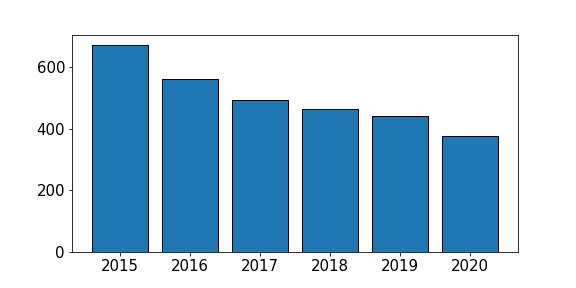
\includegraphics[scale=0.6]{img/pog_dyn_years}}
	\caption{Количество погибших в ДТП (г. Москва)}
\end{figure}

Как упоминается в \cite{kostych} согласно относительно свежим данным, есть несколько основных причин возникновения ДТП в РФ: 
\begin{itemize}
	\item нахождение детей на дороге или недалеко от нее
	\item загруженность дорог по выходным
	\item пренебрежение правилами дорожного движения водителем
	\item опрокидывание транспортного средства
	\item наезд на пешехода
\end{itemize}

Каждая вышеперечисленная причина в идеале требует отдельного анализа. Достаточно легко поверить, что не существует единого правила, которое способно ослабить риск каждого ДТП, однако верхнеуровневый анализ позволит понять некоторые самые <<проблемные>> места работа над которыми даст максимальный эффект.

Наличие актуальной статистики дорожно-транспортных происшествий, в совокупности с анализом текущей ситуации позволит государству своевременно корректировать меры и действия в рамках принятой стратегии. 

\subsection{Обзор литературы}
Существует не так много статей посвященных анализу ситуации с ДТП в России. Основной причиной для этого считаю доступность и структурированность имеющихся данных. Существующие источники являются достаточно <<сырыми>>, что осложняет задачу для написания больших аналитических работ. Однако, исследования на эту тему все-таки есть.

В \cite{ivliev_econ_stat_analysis} авторы рассматривают дорожную ситуацию на верхнем уровне, оперируя федеральными округами и областями. Авторы подмечают важность плотности дорог (площадь на 1000 км территории). Наблюдается рост этого показателя во всей Российской Федерации, однако данный рост тяжело наблюдать оперируя отдельными федеральными округами. Из работы также можно понять, что в недалеком прошлом был небольшой ежегодный рост введения дорог с твердым покрытием. Авторы подмечают, что качество дорог является важный фактором не только для снижения количества, но и для степени тяжести ДТП. На уровень транспортных происшествий также влияет количество автомобилей. По данным на конец 2013 года в Российской Федерации насчитывалось порядка 53 321 тысяч транспортных средств, при росте в $17.5\%$ по отношению к прошлому году. Для того, чтобы оценить влияние количества транспортных средств на количество случае ДТП в статье строится регрессионная модель из которой следует, что это влияние действительно есть. Более того, количество автомобилей объясняют порядка $90\%$ дисперсии случаев ДТП по разным регионам. Статья в целом посвящена итогам Федеральной целевой программы по повышению безопасности дорожного движения в 2006---2012 гг. Авторы отмечают успех данной программы, но заявляют, что ситуация на дорогах все еще требует пристального внимания со стороны правительства.

Другая, достаточно свежая статья \cite{klachkiva2020analiz} посвящена анализу статистики ДТП на уровне всей страны. Авторы также отмечают бурный рост количества автомобилей зарегистрированных в РФ, что конечно ведет к дополнительным транспортным проблемам: снижение скорости сообщения из-за большей дорожной загрузки, увеличение выбросов вредных веществ, а также перерасход топлива. В своей работе, авторы делают разрез пострадавших в ДТП по годам и подмечают, что не смотря на то, что общее количество ДТП и пострадавших в них уменьшается за последние 5 лет, существует рост количества пострадавших/погибших в ДТП детей в возрасте до 16 лет. Также авторы подмечают, что самая частая группа пострадавших в ДТП --- это люди с активным образом жизни от 21 до 40 лет. Такая ситуация, по словам авторов негативно сказывается на возрастную пирамиду населения и другие демографические показатели РФ. Авторы в своей работе отмечают снизившееся количество случаев ДТП в первую половину 2020 года, объясняя это снизившимся числом автомобилей на дороге. Однако, совсем недавно в \cite{rbkNews} отметили, что этот эффект был временным и в итоге локдаун 2020-го года никак не повлиял на количество фатальных случаев в ДТП. Как отмечают в ГИБДД, несмотря на сокращение случаев в ДТП, смертность в них, как и ситуация с вождением стала <<нестабильной>> \footnote{Стоит понимать, что данные могут разнится. В Российской Федерации актуальную информацию о случаях ДТП собирают два ведомства --- Госавтоинспеция и Росстат.}. По мнению службы, водители вновь севшие за руль после локдауна растеряли свои навыки вождения, а некоторые --- и чувство опасности, подавшись эйфории после ослабления некоторых ограничений.

В другой работе \cite{kuzmenko2020analysis} затрагивался вопрос прогнозирования вероятности ДТП с участием пешеходов. Авторы располагали похожими данным, что использовались и в данном исследовании --- карточки ДТП скачанные из сайта stat.gibdd.ru. Авторы описывают методологию сбора и построения витрины данных для последующей подачи на вход моделям машинного обучения. В работе выделяются основные факторы, которые могут иметь предсказательную силу, а также тонкостям сбора подобных данных. В качестве прогнозной модели авторы советуют использовать реализацию градиентного бустинга над деревьями Catboost --- библиотека с открытым доступом, разработанный компанией Яндекс. В статье рассказываются преимущества над существующими реализациями, а также даются рекомендации по настройке параметров модели. Авторы подчеркивают <<несовершенство>> данных в карточках ДТП, которые могут быть результатом человеческих ошибок. В качестве основной мотивации для создания подобной модели, выделяется высокая доля наездов на пешеходов, где наблюдается наивысшее среднее количество пострадавших в ДТП. Остается за кадром построение модели, как и постановка задачи.

В другой работе \cite{konyuhov2015analysis} производится анализ динамики пострадавших в ДТП. На момент исследования данных наблюдалось снижение количества пострадавших и погибших на существенных статистически значимых показателях. Авторы также приводят некоторую сводку информации по ДТП, в частности заявляя, что самыми опасными часами являются вечерние --- 30-35 \% ДТП случаются именно в этот промежуток времени. Подтверждающий эту статистику график можно увидеть в разделе обзора данных. 

В довольно ранней работе \cite{elvik2007state} рассматривают основные практики 2000-ных годов для выявления особо опасных участков дорог. На тот момент, Байесовские методы являлись основным подходом для этой задачи. Строилась некоторая модель, которая каждому участку дороги ставила в соответствие распределение количества аварий, травм, крупных происшествий и др. Полученные оценки распределений сопоставлялись с фактическими данными, после чего аномально высокие значения для распределений трактовались как проблемные места, требующие особого внимания. Ряд стран использовал схожую методологию с поправкой на вид модели, критические пороги для объявление участка дороги проблемным и подобные технические характеристики. Такой подход позволял выявлять подозрительные участки дороги, на которые впоследствии отправлялись специалисты для выявления возможной причины <<опасности>> дороги и её устранения. В работе рассматривают разные спецификации модели, а также особенности практического влияния результатов. Как говорится в статье, на тот момент Байесовский подход являлся state-of-the-art методом для подобного рода задач.


\subsection{Методология и цели}




\newpage
\bibliographystyle{utf8gost705u}  %% стилевой файл для оформления по ГОСТу
\bibliography{biblio}     %% имя библиографической базы (bib-файла) 
\end{document}
